\documentclass[twocolumn]{article}
\usepackage{PRIMEarxiv}

\usepackage[utf8]{inputenc} % allow utf-8 input
\usepackage[T1]{fontenc}    % use 8-bit T1 fonts
\usepackage{hyperref}       % hyperlinks
\usepackage{url}            % simple URL typesetting
\usepackage{booktabs}       % professional-quality tables
\usepackage{amsfonts}       % blackboard math symbols
\usepackage{amsmath}
\usepackage{amsthm}


\usepackage{natbib}

\usepackage{multirow}

\usepackage{algorithm}
\usepackage{algpseudocode}

\usepackage{nicefrac}       % compact symbols for 1/2, etc.
\usepackage{microtype}      % microtypography
\usepackage{cuted}
\usepackage{fancyhdr}       % header
\usepackage{graphicx}       % graphics
\usepackage{subfig}

\graphicspath{{images/}}     % organize your images and other figures under media/ folder

\usepackage{multicol}
\usepackage{tcolorbox}
%Header
\pagestyle{fancy}
\thispagestyle{empty}
\rhead{ \textit{ }} 

% Update your Headers here
\fancyhead[LO]{Convolution}
% \fancyhead[RE]{Firstauthor and Secondauthor} % Firstauthor et al. if more than 2 - must use \documentclass[twoside]{article}


\newtheorem*{note}{Note}
  

\newtheorem{theorem}{Theorem}
\tcolorboxenvironment{theorem}{
    colback=blue!5!white,
    boxrule = 0.2pt,
    boxsep=1pt,
    left= 2pt, right=2pt, top=2pt, bottom=2pt,
    oversize = 1.5pt,
    sharp corners, 
    before skip = \topsep,
    after skip = \topsep
}



%% Title
\title{The fast matrix composition of Pauli polynomial.
%%%% Cite as
%%%% Update your official citation here when published 
%\thanks{\textit{\underline{Citation}}: 
%\textbf{Authors. Title. Pages.... DOI:000000/11111.}} 
}

\author{
    \href{https://orcid.org/0000-0002-4876-7820}{
        
\includegraphics[scale=0.06]{orcid.pdf}\hspace{1mm}Hyunseong Kim}\\
  Department of Physics and Photon Science,  \\
  Gwangju Institute of Science and Technology\\
  Gwangju\\
  \texttt{qwqwhsnote@gm.gist.ac.kr} \\
  %% examples of more authors
  %% \AND
  %% Coauthor \\
  %% Affiliation \\
  %% Address \\
  %% \texttt{email} \\
  %% \And
  %% Coauthor \\
  %% Affiliation \\
  %% Address \\
  %% \texttt{email} \\
  %% \And
  %% Coauthor \\
  %% Affiliation \\
  %% Address \\
  %% \texttt{email} \\
}

\begin{document}
\twocolumn[ 
\begin{@twocolumnfalse}
    \begin{center}

    \maketitle

\begin{abstract}

%===== 1st Abstract ====
% We studied the relationship between a proper coefficient matrix and XZ-simplex representation of
% each Pauli terms to manipulate Hamiltonian as Pauli polynomial. Based on Tensoried decomposition
% algorithm by Hantzko et al, the simplex representation is a specific index of the coefficient matrix
% depending on the chosen basis. A binary conversion between the element index and the simplex
% representation was proposed and the composition algorithm for matrix representation of Pauli-
% polynomial based on the coeeficient matrix was designed. Importantly, our algorithm applies to
% coefficient matrices that represent complete Pauli polynomials, not merely single Pauli terms. This
% approach significantly reduces computational costs in the matrix conversion routine compared to
% previous term-by-term methods.

%===== 2nd Abstract ====
% In this research, we studied a proper coefficient matrix 
% representation for a Pauli polynomial, and its construction method. 
% The matrix could represent group structure of Pauli group more efficiently,
% than common computational basis in quantum computation.
% Thus, we get fast manipulation and analysis routines of the given Hamiltonian as Pauli polynomial.
% Based on Tensoried decomposition algorithm by Hantzko et al,
% the coefficient matrix could be transformed to computational basis representation.
% Comparing to previous term-by-term methods, 
% the method requires half time-complexity for the worst case.
% In addition, since the required spatial complexity also reduced to single $2^n \times 2^n$ elemets,
% practical time cost also smaller than the term-by-term methods.
% However, there is a weakness in composition speed for $k<4^n$ number polynomial.
% Therefore, an effective term chasing algorithm was designed. 
% By choosing these methods, researchers could accelerate the conversion between 
% Pauli terms and their matrix representation.
%time cost 

In the research, we explored the proper coefficient 
matrix for Pauli polynomials focusing on enhancing the 
group structure representation. 
With coefficient elements and thier indexes on the matrix,
we can simultaneously manipulate the group and linear structure,
more efficiently than the standard matrix representation of Pauli terms.
The construction of the matrix is based on XZ simplex representation of 
each Pauli terms in the polynomial. 
Moreover, Pauli polynomial could be represented with a single complex matrix.
We investigated two composition algorithms based on the coefficient matrix and 
tensorized decompositon algorithm suggested by Hantzko et al\cite{hantzko_tensorized_2023}.
One is a naive basis transformation in each tensor producted spaces.
The other is a modified transformation with effective term chasing routine.
The composition time and spatial complexity 
of the investigated naive algorithms is atmost $\frac{1}{2}8^n$, and $4^n$, respectively.
Since, the coefficient matrix already contains all information of the terms
in the polynomial, it is more efficient than general term-by-term construction methods, which have 
$k*(f(n)+4^n)\leq 16^n + 4^n(f(n)-1)$ time complexity and $2*4^n$ spatial complextity, where $f(n)$ is a time complexity of 
single term construction method.
\end{abstract}

% keywords can be removed
\keywords{Matrix composition \and Pauli polynomial \and Tensor product}
    \end{center}
\end{@twocolumnfalse}
]

%\begin{multicols*}{2}
    

\section{Introduction}
%This research demonstrates the proper mapping of Pauli terms from their simplex representation to the coefficient matrix and its fast composition to the matrix form. 
%The coefficient matrix is a proper basis representation of the Pauli polynomial preserving the coefficients of the corresponding Pauli terms. 
%By using the mapping from the simplex representation of Pauli terms and the coefficient matrix, we can manipulate Pauli terms more efficiently in the matrix vector space.

% In the quantum computing, a conversion between 
% Hamiltonian and Pauli polynomial is one of the fundamental routine for analysis of 
% the given system and construct the evolution operator and optimization.%\cite{}.

In quantum computing, converting between the Hamiltonian and Pauli polynomials is fundamental 
for both analyzing the system and constructing the evolution operator and its optimization.
Since the Pauli polynomial indicates the local structures of the system,
and Hamiltonian with Hermitian matrix form shows overall characteristics.
% What is an "overall characteristics".

\begin{equation}
    H = \sum_i^n \lambda_i P_i
\end{equation}

Therefore, if the Hamiltonian is represented by a Hermitian matrix, 
a decomposition is required to get the coefficients of the terms. 
On the other hand, if the Pauli polynomial is given, 
one needs to construct Hermitian matrix by linear combinations of each term and condition.
This process is called \textit{composition}.
Since, the Pauli matrices and their tensor products form an orthonormal basis 
of $2^n \times 2^n$ matrix Hilbert space\cite{nielsen2010quantum}, 
the decomposition and composition are well-defined with Hilbert-Schmidt inner product. 

\begin{equation}
    \label{eq:pauli_group}
    \sigma_0 = I, 
    \sigma_1 = \begin{bmatrix}
        0 & 1 \\
        1 & 0 \\
    \end{bmatrix},
    \sigma_2 = \begin{bmatrix}
        0 & -i \\
        i & 0 \\
    \end{bmatrix},
    \sigma_3 = \begin{bmatrix}
        1 & 0 \\
        0 & -1 \\
    \end{bmatrix}
\end{equation}

%-------------------------------------------
There are well-known matrix representation of basic Pauli algebra, see Eq(\ref{eq:pauli_group}).
In higher dimensions, the $n$-fold Pauli terms are represented with a tensor producted terms of the above single Pauli-matrices. 
However, in larger systems, the usage of the common matrix representation requires too much computational costs 
for its group and linear structures. 

A simplex representation could be a solution of the problem. 
It maps each Pauli term to geometrical language of symplectic polar spaces\cite{havlicek_moebius_2009}.
There are several ways to map the each tern to the simplex representation, 
however, a common method is using a XZ family string representing Pauli term as product of two Pauli terms whose elements are only I, X or I, Z.
The representation is expressed as a positive integer tuple by decompose the product string as matrix product of X, Z family strings.
It is possible to implement the well-define binary operation for Pauli-group algebra.
Since, the algebra implementation on matrix space have huge operational complexity comparing to 
single integer or binary operation, the simplex representation and their algebra implementation 
provide us a lot of convenience for generating and manipulating of the terms efficiently in computation frameworks.
For example, Reggio et al showed that we can accelerate a determination of their commutation relationship 
with their simplex representation\cite{reggio_fast_2023}.

However, the manipulation and properties of Pauli terms does not only live in group structure. 
Hamiltonian analysis is also based on their vector property on complex field. 
Meanwhile, the simplex representation itself does not provide a linear structure
of the Pauli basis in matrix space.
One solution is constructing a single matrix which is a summation of all Pauli terms in their matrix form.% 연결을 더해라
Therefore, it is also an intense of study that the fast construction of a $n$-fold Pauli matrix from single pauli string, 
or simplex representations or decomposition of the given matrix into Pauli polynomials.
There have been some studies about fast decomposition\cite{hantzko_tensorized_2023, koska_tree-approach_2024, ying_preparing_2023} %\cite{} decomposition papers
and composition\cite{vidal_romero_paulicomposer_2023} routines,%\cite{} composition papers 
when a system is given with a hermite matrix, a set of coefficient, or a single Pauli string.

Another solution is allocating standard basis to each Pauli term, to indicate their 
linear structure. Since, Pauli matrices are orthonormal basis with Hilbert-Schmidt inner product\cite{nielsen2010quantum},
the mapping is well-defined. However, what is a proper basis mapping, that is useful to manipulate their group and linear 
struture simultaneously, is a questionable. 
The standard basis has a lot of convenience, since, it is not only indiciating of the linear structure, 
but also, preserves coefficient and Pauli terms in Pauli polynomial, as value and index of the elements. 

Therefore, in this paper, we proposed a proper coefficient matrix 
to be used in Pauli polynomial representation.
The matrix construction from simplex representations, 
and conversion methods to computational basis were investigated. 
The noticiable work in the previous studies is a tensorized pauli decomposition(TPD) algorithm studied by Hantzko et al\cite{hantzko_tensorized_2023}.
The coefficient matrix refer in the paper is came out as a result of TPD algorithm.

In the following sections, we showed that the TPD is just a basis transformation 
represented with sequential local operations of the tensor producted spaces. 
By their property, unitary, it is automatically achieved the existence of inverse transformation.
Lastly, a simple conversion operation was suggested that mapping between a simplex representation and index of the coefficient matrix
of Pauli terms.
With these knowledges, the coefficient matrix could be used for representing group and linear structure 
of Pauli matrices in general $n$-fold Pauli terms, fascillating fast conversion between matrix and its pauli decomposition.
The main advantage of the coefficient matrix in composition routine is that the term by term construction and summation is not 
needed to build matrix representation of the Pauli polynomial. The summation is already archieved in the coefficient matrix, 
and the time complexity of the algorithm does not depend on the number of terms of the polynomial. 


\section{Background knowledges}

%\subsection{Pauli matrices and terms}

\subsection{Simplex representation}

If we use $\sigma'_2$ as one of pauli basis, where $\sigma_2 = i \sigma'_2$,
and seperate phase to the outside,
the tensor producted representation of $n$-fold Pauli terms has a next form.

\begin{equation}
    P_{g} = \{\sigma_0 , \sigma_1, \sigma'_2, \sigma_3\}
\end{equation}

\begin{equation}
    P = (i)^m \otimes_j^n \sigma_j
\end{equation}

where, $m$ is a number of occurrence of $\sigma'_2$ in the product.
Since $\sigma'_2 = \sigma_1 \sigma_3$ holds true, we can decompose the given $n$-fold Pauli term as next two
parts; elements of families. 
The example families are $z$-family and $x$-family refered by Reggio et al\cite{reggio_fast_2023}.

\begin{equation}
    \label{eq:xz_decompose}
    \otimes_j^n \sigma_j = \left( \otimes_{j \in \{0, 1\}}^n \sigma_j \right) \left( \otimes_{k \in \{0, 3\}}^n \sigma_k \right)
\end{equation}

Eq(\ref{eq:xz_decompose}) yields an unique representation as integer tuple of length 2 by 
replace $I \rightarrow 0, X, Z \rightarrow =1$ in the each memebers.

\begin{equation}
    P = (n_x, n_z)
\end{equation}

where $n_x, n_z$ are integers whose binary representation indicates $I=0, X=1, Z=1$.

For example, $(6, 5)$ of 3-qubit system is a simplex representation of $\text{YXI}$.

\begin{equation}
    \begin{array}{c}
        6 = 1 \cdot 2^2 +1 \cdot 2^1 + 0 \cdot 2^0 = X \otimes X \otimes I\\
        5 = 1 \cdot 2^2 +0 \cdot 2^1 + 1 \cdot 2^0 = Z \otimes I \otimes Z
    \end{array}
\end{equation}


IBM implemented the above simplex representation 
for their \textit{Pauli} class in python library, \text{Qiskit},
to use the above binary implementation\cite{Qiskit}. 
However, in the paper, the order of the simplex representation 
is reversed order of the IBM implementation. 
There is no difference in algebra implementation and 
commutation conversion routine, however, the conversion to index of coefficient
matrix is more direct in the reversed order than the IBM order.

\subsection{Tensorized decomposition}

In 2023, Hantzko et al showed that 
general $\mathbf{M}_{2^n}(\mathbb{C})$ matrices are efficiently decomposed into 
several Pauli terms with corresponding coefficients, using a tensorized notation\cite{hantzko_tensorized_2023}.

\begin{equation}
    \sum_{i=0}^3 c_i \sigma_i = 
    \begin{bmatrix}
        A_{11} & A_{12}\\
        A_{21} & A_{22}
    \end{bmatrix}
    \rightarrow_{TPD}
    \begin{bmatrix}
        c_0 & c_1\\
        c_2 & c_3
    \end{bmatrix}
\end{equation}

where, 
\begin{equation}
    \label{eq:tpd_transform}
    \begin{array}{ccc}
        A_{11} & = &  c_0 + c_3\\
        A_{12} & = &  c_1 - i c_2\\
        A_{21} & = &  c_1 + i c_2\\
        A_{22} & = &  c_0 - c_3.
    \end{array}
\end{equation}

The basic idea is decoupling the coefficients of each tensor producted space, iteratively. 
See Figure \ref{fig:tpd_diagram}.

\begin{figure}[!h]
    \centering
    \includegraphics*{images/tpd_diagram.pdf}
    \caption{Iterative diagram of Tensorized Pauli Decomposition algorithm.}
    \label{fig:tpd_diagram}
\end{figure}

In their implementation, they did not map the index of the result cofficient matrix to 
each Pauli term. Therefore, they mapped the coefficients by adding a character to each string variables 
in each step of the iteration. 

The decomposition process is non-linear in $2^n \times 2^n$ matrix space. 
However, it is a basis transformation in a higher dimension $\mathbb{C}^N$ space, 
which is isomorphic to the vector spaces with $N = 4^n$ dimension.

For example, the $2 \times 2$ dimension matrix of 1 qubit system, the process could be expressed as 
$\mathbf{v} \in \mathbb{C}^4$. 

\begin{equation}
    \frac{1}{2}
    \begin{bmatrix}
        1 & 0 &  0 &  1\\
        0 & 1 &  1 &  0\\ 
        0 & i & -i &  0\\ 
        1 & 0 &  0 & -1 
    \end{bmatrix}_{TPD}
    \begin{bmatrix}
        A_{11} \\
        A_{12} \\
        A_{21} \\
        A_{22}
    \end{bmatrix} =
    \begin{bmatrix}
        c_0\\
        c_1\\
        c_2\\
        c_3
    \end{bmatrix}
\end{equation}

In $2 \times 2$ matrix with computational basis, the next matrix is a \textit{coefficient matrix} of 1 qubit system.

\begin{equation}
    \begin{bmatrix}
        c_0 & c_1\\
        c_2 & c_3
    \end{bmatrix}
\end{equation}

In the vectorized representation, the intermiediate step of TPD algorithm 
could be represented with the next notation. 

\begin{eqnarray}
    &\begin{bmatrix}
        A_{11} \\
        A_{12} \\
        A_{21} \\
        A_{22}
    \end{bmatrix}_1 \otimes
    \begin{bmatrix}
        A_{11} \\
        A_{12} \\
        A_{21} \\
        A_{22}
    \end{bmatrix}_2 \otimes
    &\cdots \otimes
    \begin{bmatrix}
        A_{11} \\
        A_{12} \\
        A_{21} \\
        A_{22}
    \end{bmatrix}_{n-1} \otimes
    \begin{bmatrix}
        A_{11} \\
        A_{12} \\
        A_{21} \\
        A_{22}
    \end{bmatrix}
    \nonumber\\
    & &\Downarrow_{i \text{steps}, i>2} \label{eq:vec_tpd}\\
    &\begin{bmatrix}
        c_0\\
        c_1\\
        c_2\\
        c_3
    \end{bmatrix}_1 \otimes
    \begin{bmatrix}
        c_0\\
        c_1\\
        c_2\\
        c_3
    \end{bmatrix}_2 \otimes
    &\cdots \otimes
    \begin{bmatrix}
        A_{11} \\
        A_{12} \\
        A_{21} \\
        A_{22}
    \end{bmatrix}_{n-1} \otimes
    \begin{bmatrix}
        A_{11} \\
        A_{12} \\
        A_{21} \\
        A_{22}
    \end{bmatrix}_n\nonumber
\end{eqnarray}

For the $n$-fold matrix, the researcher can choose the basis trnasformation, freely.
The transformation even permits the different basis in each producted and each sub-matrix
operations. The result coefficient matrices have identical coefficients without considering indexing.
By choosing appropriate basis, the decompositon yields the Latin matrix whose element indexes are XZ simplex representation
of Pauli terms in Reggio et al\cite{reggio_fast_2023}.
In below sections, we refer the index of coefficients as \textit{ij-index} in the result matrix 
by basis transformation refered from Hantzko et al.

\section{Simplex to Coefficient map}

The mapping could be vary in general cases, however for convenience, we only consider
the general XZ simplex representation by Reggio et al\cite{reggio_fast_2023} and 
ij-index generated from \cite{hantzko_tensorized_2023}.
It is possible to use XZ representation as an index of Pauli terms, 
however, there is an efficient issues.
T he XZ index is well-organized for group structure and 
the ij-index has a benefit in computational cost in decomposition and composition.
By the object of the Pauli manipulation, the proper index could be different.

With these two representation of the same Pauli term, the next relationship is achieved.

\begin{theorem}
    For a given simplex representation, $(n_x, n_z)$ of the given Paili term, $P$,
    their index, $(i, j)$, in coefficient matrix is determined as 
    $$(i, j) = (n_z, n_x^\wedge n_z)$$

    where, ${}^\wedge$ is a XOR bitwise operator. 
\end{theorem}

\textbf{Proof} 
From $i$-th iteration of the TPD algorithm of $2^n$ dim square matrix, 
the unit sub-matrix dimension is $2^{n-i}$ and there are 4 block matrices, see Figure \ref{fig:tpd_diagram}.
With Eq(\ref{eq:xz_decompose}), the result matrix of $i-th$ iteration is

\begin{equation}
    \begin{bmatrix}
        \sigma_0 \cdot \sigma_0 & \sigma_1 \cdot \sigma_0\\
        \sigma_1 \cdot \sigma_3 & \sigma_0 \cdot \sigma_3\\
    \end{bmatrix}
    = 
    \begin{bmatrix}
        0_x \cdot 0_z & 1_x \cdot 0_z\\
        1_x \cdot 1_z & 0_x \cdot 1_z\\
    \end{bmatrix}
\end{equation}

where, $0_z, 1_z, 0_x, 1_x$ are XZ binary representation of Pauli term of $i$-th decimal.
For row index, $2^{i} * nz_i, nz_i\in \{0_z, 1_z\}$ the Z-binary determine
the row index movement, if $nz_i = 1_z$, the row location is changed else it is not.
For column index, the column index changed by $+0$ if $(1_x, 0_z)$ or $(0_x, 1_z)$, 
else $+2^{n-i}$ if $(0_x, 0_z)$ or $(1_x, 1_z)$.
It is a simple XOR binary opertor, therby 
$2^{n-i} * nz_i^{\wedge}nx_i, \, nz_i\in \{0_z, 1_z\}, nx_i \in \{0_x, 1_x\}$

Thus, we have (i, j) coefficient index of XZ representation by iteration from 1-th to $n$-th. 

\begin{equation}
    \begin{array}{clcc}
    i =& \sum_{k=0}^{n-1} 2^{k} nz_k &=& nz\\
    j =& \sum_{k=0}^{n-1} 2^{k} nz_k^{\wedge} nx_k &=& nz^{\wedge}nx
    \end{array}
\end{equation}

where $nz_k, nx_k$ are $k$-th binary element of $nz, nx$ binary representation of the given Pauli term $\square$.

With this relationship, we can construct a matrix representation of the given Pauli polynomial
by inversing TPD algorithm. 
The terms would be located in corresponding elements in 
the coefficient matrix and the inverse composition algorithm would generate the original matrix.

\subsection{Inverse algorithm}

In the previous section, we already showed that TPD algorithm is a sequential 
applying of unitary transformation for each vectors in a product representation.
By the property of unitary, the inverse transformation is well defined 
in $4^n$ dimension and we can implement it in $2^n$ with 
sub-block matrix additions. 
The $\{c_i\}_{i=0}^3$ coefficients in Eq (\ref{eq:tpd_transform}) is restored as 

\begin{equation}
    \label{eq:restore}
    \begin{array}{ccc}
        c_0 &=& \frac{1}{2} (A_{11} + A_{22})\\
        c_1 &=& \frac{1}{2} (A_{12} + A_{21})\\
        c_2 &=& \frac{i}{2} (A_{12} - A_{21})\\
        c_3 &=& \frac{1}{2} (A_{11} - A_{22})\\
    \end{array}
\end{equation}.

The composition is achieved by iteratively applying the Eq (\ref{eq:restore}) in reverse order of TPD algorithm. 
See, Fig (\ref{fig:tpd_diagram}).

\begin{algorithm}
    \caption{Naive Inverse Composition Algorithm}\label{alg:naive_inverse}
    \begin{algorithmic}
        %\Require poly = $\{(c_i, (nx_i, nz_i))\}_{i=1}^k$
        %\Require n = Tensor Product dimension \Comment{Qubit number}
        %\Comment{Conversion to ij index}
        %\State polyij $\gets$ [] 
        %\For{ i \textbf{in} range(k)}
        %    \State $c_i \gets$ poly[i].c
        %    \State $nx_i \gets$ poly[i].nx
        %    \State $nz_i \gets$ poly[i].nz
        %    \State{polyij[i] $\gets (c_i, (nz_i, nx_i^\wedge nz_i))$ } 
        %\EndFor
        %\Comment{Construct coefficient matrix}
        %\State $M \gets $ Zero matrix of ($2^n$, $2^n$).
        %\For{c, i, j \textbf{in} polyij}
        %    \State{M$[\text{i}][\text{j}]$ = c} 
        %\EndFor
        \Require $M \gets$ Coefficient matrix of $(2^n, 2^n)$
        \State matdim $\gets 2^n$
        \State steps $\gets$ n
        \State unit\_size $\gets$ 1

        \For{step \textbf{in} steps}
            \State step1 $\gets$ step+1
            \State mat\_size $\gets 2*\text{unit\_size}$
            \State indexes $\gets$ [matdim/$2^{\text{step1}}$]
            \State indexes\_ij $\gets$ mat\_size*indexes
            \For{i \textbf{in} indexes\_ij}
                \For{i \textbf{in} indexes\_ij}
                \State $r_{1s}\gets$ i
                \State $r_{1f2s}\gets$ $r_{1s}$ + unit\_size
                \State $c_{1s}\gets$ j
                \State $c_{1f2s}\gets$ $c_{1s}$ + unit\_size
                \State $r_{2f}\gets$ $r_{1f2s}$ + unit\_size
                \State $c_{2f}\gets$ $c_{1f2s}$ + unit\_size

                \State coef $\gets$ 1

                \State $M$[$r_{1s}$: $r_{1f2s}$, $c_{1s}$:$c_{1f2s}$] += coef*$M$[$r_{1f2s}$: $r_{2f}$, $c_{1f2s}$:$c_{2f}$]
                \State $M$[$r_{1f2s}$: $r_{2f}$, $c_{1f2s}$:$c_{2f}$] = $M$[$r_{1s}$: $r_{1f2s}$, $c_{1s}$:$c_{1f2s}$] -2*coef *$M$[$r_{1f2s}$: $r_{2f}$, $c_{1f2s}$:$c_{2f}$]

                \State coef $\gets - \sqrt{-1}$ 
                \State $M$[$r_{1f2s}$: $r_{2f}$, $c_{1s}$:$c_{1f2s}$] += coef*$M$[$r_{1s}$: $r_{1f2s}$, $c_{1f2s}$:$c_{2f}$]
                \State $M$[$r_{1s}$: $r_{1f2s}$, $c_{1f2s}$:$c_{2f}$] = $M$[$r_{1f2s}$: $r_{2f}$, $c_{1s}$:$c_{1f2s}$] -2*coef *$M$[$r_{1s}$: $r_{1f2s}$, $c_{1f2s}$:$c_{2f}$]
                
                \EndFor
            \EndFor
            \State unit\_size $\gets$ 2*unit\_size
        \EndFor
    \end{algorithmic}
\end{algorithm}

The important of the algorithm is that 
the maximum time complexity is same between one pauli term and general pauli-polynomial.
In addition, as has mentioned in \cite{hantzko_tensorized_2023}, it does not need further 
instant matrix to save the terms, so that spatial complexity of the algorithm is also practical 
in large system.
See details in the below complexity analysis section.

\subsubsection{Effective term chasing algorithm}

If we know an index set of Pauli terms, where their coefficients are not zero,
we could avoid the operation for zero sub matrices terms in the intermediate steps of the composition.
The non zero terms is denoted with \textit{effective} terms. 
Considering I-Z and X-Y calculation, when $k$ number of Pauli terms were given, 
there is an $k_{eff}$ number of effective terms where

\begin{equation}
    k = k_{eff} + d\, d \geq 0
\end{equation}, $d$ is a number of the duplicated terms.

From the $i$-th effective index set, the effective index set for the next step is calculated by
quotient of 2, such as 

\begin{equation}
    \label{eq:term_chasing}
    \begin{array}{ccc}
        row_{i+1}&=& r_i \\
        col_{i+1}&=& c_i
    \end{array}
\end{equation}

where, $row_i = 2*m_i + r_i$ and $col_i = 2*n_i + c_i$.
The $k_i$ number is same with $(k_{eff})_{i-1}$ number. 

For example, in $2^4 \times 2^4$ coefficient matrix, 
if we have 
(1, 14), 
(2, 13), 
(3, 1), 
(6, 4),
(7, 4),
(7, 5),
(13, 9),
(14, 10) elements 
were non-empty Pauli terms. 
We can chasing the non empty unit indexes with Eq (\ref{eq:term_chasing})

\begin{equation}
    \begin{array}{lccccc}
                & (1, 14)     & (0, 7)   &  (0, 3)& (0,1)&(0,0)\\
                & (2, 13)     & (1, 6)   &  (0, 0)& (0,0)&\\
                & (3, 1)      & (1, 0)   &  (1, 1)& (1,1)&\\
                & (6, 4)      & (3, 2)   &  (3, 2)& -    &\\
                & (7, 4)      & (6, 4)   &  -     & -    &\\
                & (7, 5)      & (7, 5)   &  -     & -    &\\
                & (13, 9)     & -        &  -     & -    &\\
                & (14, 10)    & -        &  -     & -    &\\
       k        & 8           & 6        &  4     & 3    & 1\\
       k_{eff}  & 6           & 4        &  3     & 2    & 1
    \end{array}
\end{equation}.

See \ref{alg:effective_terms} for further details.

%See details in appendix 2. %Computational details.

\begin{algorithm}
    \caption{Effective term algorithm}\label{alg:effective_terms}
    \begin{algorithmic}
        \Require poly = $\{((i, j))\}_{l=1}^k$ \Comment{ij converted Pauli terms}
        \Require $M \gets$ Coefficient matrix of $(2^n, 2^n)$
        \State matdim $\gets 2^n$
        \State steps $\gets$ n
        \State unit\_size $\gets$ 1
        
        \For{step \textbf{in} steps}
            \State pstep $\gets$ [] \Comment{Empty list}
            \State dup   $\gets$ []
            \For{(i, j) \textbf{in} poly}
                \If{(i, j) \textbf{in} dup}
                    continue
                \EndIf
                %\State pclass $\gets$ (i+j)\%2
                \State n, o $\gets$ i\%2, j\%2  \Comment{IZ, XY determination}
                \State l, m $\gets$ (i+1-2*(n), j+ 1-(2*(o))) \Comment{Get a corresponding location}
                
                \State dup.insert((l,m) , (i,j))
                
                \If{ n == 1}
                    \State pair $\gets$ ((l, m), (i, j))
                \Else
                    \State pair $\gets$ ((i, j), (l, m))
                \EndIf

                \If{ (i+j)\%2 == 1}
                    \State coef $\gets - \sqrt{-1}$ 
                \Else
                    \State coef $\gets 1$
                \EndIf

                \State $r_{1s}\gets$ unit\_size * pair[0][0]
                \State $r_{1f}\gets$ $r_{1s}$ + unit\_size
                \State $c_{1s}\gets$ unit\_size * pair[0][1]
                \State $c_{1f}\gets$ $c_{1s}$ + unit\_size

                \State $r_{2s}\gets$ unit\_size * pair[1][0]
                \State $r_{2f}\gets$ $r_{2s}$ + unit\_size
                \State $c_{2s}\gets$ unit\_size * pair[1][1]
                \State $c_{2f}\gets$ $c_{2s}$ + unit\_size

                \State $M$[$r_{1s}$: $r_{1f}$, $c_{1s}$:$c_{1f}$] += coef*$M$[$r_{2s}$: $r_{2f}$, $c_{2s}$:$c_{2f}$]
                \State $M$[$r_{2s}$: $r_{2f}$, $c_{2s}$:$c_{2f}$] = $M$[$r_{1s}$: $r_{1f}$, $c_{1s}$:$c_{1f}$] -2*coef *$M$[$r_{2s}$: $r_{2f}$, $c_{2s}$:$c_{2f}$]

                \State i >>=1 \Comment{Bit shift operation}
                \State j >>=1

                \If{(i, j) \textbf{in} pstep}
                    continue
                \Else:
                    pstep.insert((i,j))
                \EndIf
            \EndFor
            \State poly $\gets$ pstep
            \State unit\_size $\gets$ 2*unit\_size
        \EndFor
    \end{algorithmic}
\end{algorithm}




\section{Comparsion to other method}

\subsection{Complexity analysis}

\subsubsection{Term-by-term methods}

The general Pauli-composition methods focus on 
term-by-term matrix implementation. That is, with the given 
$k$-term Pauli polynomial, the previous methods generate $k$ matrices corresponding to 
each tern and sum the matrices.

For $2^n \times 2^n$ matrices, if we denote the complexity of an algorithm for constructing a single Pauli matrix,
$f(n)$, then the total composition complexity is estimated as,

\begin{equation}
    \label{eq:k-complexity}
    k * f(n) + (k-1) 4^n
\end{equation}

where the $4^n$ term represents element wise addition complexity.
Since $k$ ranges from 1 to $4^n$, the maximum complexity is

\begin{equation}
    \label{eq:max_complexity}
    16^n + 4^n(f(n)-1)
\end{equation}

therefore, the term-by-term algorithms are fast with atmost $16^n$ time-complexity.
% 여기 알고리즘 시간 복잡도 설명 더 쓰고 공간 복잡도도 같이 쓰자
Spatial complexity of temr-by-term methods is $2 \cdot 4^n$ by preparing 
zero matrix and iteratively adding each terms to the zero matrix.

\subsubsection{Algorithm complexity}

In the naive algorithm \ref{alg:naive_inverse},
the time complexity of each step is $4^n$, and there are $2^{n-1}$ 
number of steps. Therefore, the total time complexity is 

\begin{equation}
    2^{n-1} 4^n = \frac{1}{2}8^n
\end{equation}

For the effective term algorithm,
it is very complicated for estimating time-complexity,
however, by taking worst case of effective term, we can estimate its upper bound.

With initial $k = k_{eff} +d$ number non zero-terms,
the most hardness of the estimation is came out from the varying 
of the effective term numbers in the iteration.
We assume that the worst case that $d=0$ and we ignore the 
steps where the all elements is non zero.
With the assumptions, we have 

\begin{equation}
    k_{eff, 0} \in [\frac{1}{2}4^{n}], k_{eff, i} = \frac{1}{2} k_{eff, i-1}
\end{equation}

with duplication search step of $O(k_{eff, i})$ complexity,
the total time complexity consists of 

\begin{equation}
    \label{eq:t_com_eterm}
    2 n * k_{eff}^2 + 34 (2^{n+1} -1) k_{eff}
\end{equation} 

The maximum complexity is not different in the naive version but it is still
lower than any term-by-term algorithm. About the effective term algorithm,
at some range of $k_{eff}$ value it is the most efficient but 
at very small or worts case, the naive version is more efficient. 
The worst complexity of the effective algorithm arises 
when $k=\frac{1}{2}4^n$ so that,

\begin{equation}
    \frac{n}{2} 16^n + 17 (2 * 8^n - 4^n) 
\end{equation}.

From Eq (\ref{eq:t_com_eterm}), the benefit region to use 
the effective term algorithm is 

\begin{equation}
    k < \frac{1}{2n} \left(\sqrt{289(2^{n+1})^2 + n 8^n} - 17 (2^{n+1} -1) \right) 
\end{equation}

The efficient is archieved when the non zero terms are under 0.5\% of $4^n$ number of terms.

\begin{table*}
    \centering
    \caption{Summary of complexity of the algorithms with big-O notation.}
    \label{table:complexity}
    \begin{tabular}{l|l|cc}
        -                                & Case      & Time complexity                   & Spatial complexity\\
        \hline
        \multirow{2}{8em}{Term by term}  & Common    & $O(k(f(n) +4^n))$                 & \multirow{2}{2em}{$O(4^n)$}\\
                                         & Worst     & $O(16^n)$                         &\\
        \multirow{2}{8em}{Naive}         & Common    &\multirow{2}{1em}{$O(8^n)$}        & \multirow{4}{2em}{$O(4^n)$}\\
                                         & Worst     &                                   &\\
        \multirow{2}{8em}{Effective term}& Common    &$O(n * k_{eff}^2)$                 & \\
                                         & Worst     &$O(n16^n)$                         & \\
        \hline                                      
    \end{tabular}
\end{table*}


\subsection{Benchmarks with the other frameworks}

The belows are brief reviews of current quantum frameworks.
List of the fraameworks and methods are provides Pauli composition routine.

\begin{itemize}
    %\item Tree approach algorithm\cite{koska_tree-approach_2024}. % decomposition 이지만, composition도 지원.
    \item PauliComposer\cite{vidal_romero_paulicomposer_2023}.
    \item Qiskit Pauli, to\_matrix method \cite{Qiskit}.
    \item Pennylane, Pauli to matrix \cite{bergholm2018pennylane}. %  https://docs.pennylane.ai/en/stable/code/api/pennylane.pauli.pauli_word_to_matrix.html
    \item Cirq: unitary matrix transform \cite{cirq_developers_2023_10247207}. %https://quantumai.google/reference/python/cirq/PauliString and further unitary matrix routine.
\end{itemize}

Pennylane and Cirq's matrix conversion are just a simple kronecker product of each matrix terms.
In the recent version of Pennylane, they provide \textit{PauliSetence} class and matrix routine.
However, the current implementation is not stable for test the general matrix composition.%Pennylane routine review

Meanwhile, Qiskit routine is based on X, Z simplices representation of Pauli term 
and they implemented the composition routine with PauliComposer method 
which uses row wise mapping.
They provides \textit{PauliList} class aslike in Pennylane. 
The \textit{to\_matrix} routine generates rank-3 matrices for the given Pauli terms.
However, the class does not support coefficient supports. 
The composition needs alternative summation with coefficient multiplication.

The main conversion were conducted with 4 implementations the inverse tensorized algorithm
with using efficient term chasing routine or not, or pure python-numpy routine and numba acceleration.

Therefore, the comparsion with naive tensor product method and PauliComposer method
is enough to see Pennylane and Qiskit frameworks. 
About the comparsion, the each routines are prepared as their intended 
data. For example, Pennylane prepares the single Pauli term as Pauli object class
, and Qiskit requires them to be in the simplex representation.

The estimation was conducted for $n$-qubit system random matrices from $n=1$ to $n=9$
with 20\%, 40\%, 60\%, 80\%, 100\% terms of $4^n$ polynomial.
In the previous section we already showed that the effective term algorithm is 
efficient when only 0.5\% terms are non zero in the space, however,
for the practical application, we started from 20\% non zero terms. 
The system specification and libraries are denoted on Table \ref{table:specs}


\begin{table}[h]
    \centering
    \caption{System specification for simulation.}
    \label{table:specs} 
    \begin{tabular}{p{2.2cm}p{4.2cm}}
    \hline 
     Processor      & {AMD Ryzen 5 1600, \newline{Six-Core Processor, 3.20 GHz}}\\ 
     RAM            & {32.0 GB}                     \\  
     OS             & {Windows 10 Home, 64bit, 22H2}\\ 
     Python         & {3.11.8} \\
     Numpy\cite{harris2020array} & 1.26.4\\
     Scipy\cite{2020SciPy-NMeth} &  1.13.0 \\
     Qiskit\cite{Qiskit}         & 1.0.2  \\  
     Pennylane\cite{bergholm2018pennylane}  &  0.35.1 \\
     PauliComposer\cite{vidal_romero_paulicomposer_2023} & Original paper version.  \\ % Fixed column spanning syntax
    \hline
    \end{tabular}
\end{table}


\subsection{Results}

In Fig (\ref{fig:results}), we tested the Pauli-composition methods in various quantum frameworks.
There was no method considering Pauli-polynomials for matrix conversion, so that all the methods are 
term-by-term methods.
\textit{paulicomposer} has a $f(n) = 2^n$ time complexity, therefore, the total composition complexity is 
$8^n$ and standard tensor product method has $f(n) = 4^n$ time complexity, so that the total complexity is 
$2 \cdot 8^n - 4^n$.

The naive algorithm showed most efficient time costs for higher $n>6$ system for all cases.
It took $10^{1}$ or $10^{3}$ times faster than term-by-term methods. 
Even in the smaller system $n<5$, the time costs were compatible with the term-by-term methods.
The effective term algorithm showed better time costs in $n<5$ and the non-zero terms accounted for
the matrix below 60\% percentage of the whole system. 
however, comparing to the naive algorithm there was no significant time benefit for the 
term chasing, it can be adopted to further applications but in the current stage, 
the improvement was not noticiable. Moreover, in the higher dimension system 
it overwhelms the term-by-term methods.

\begin{figure*}[ht]
    \centering
        \subfloat[]{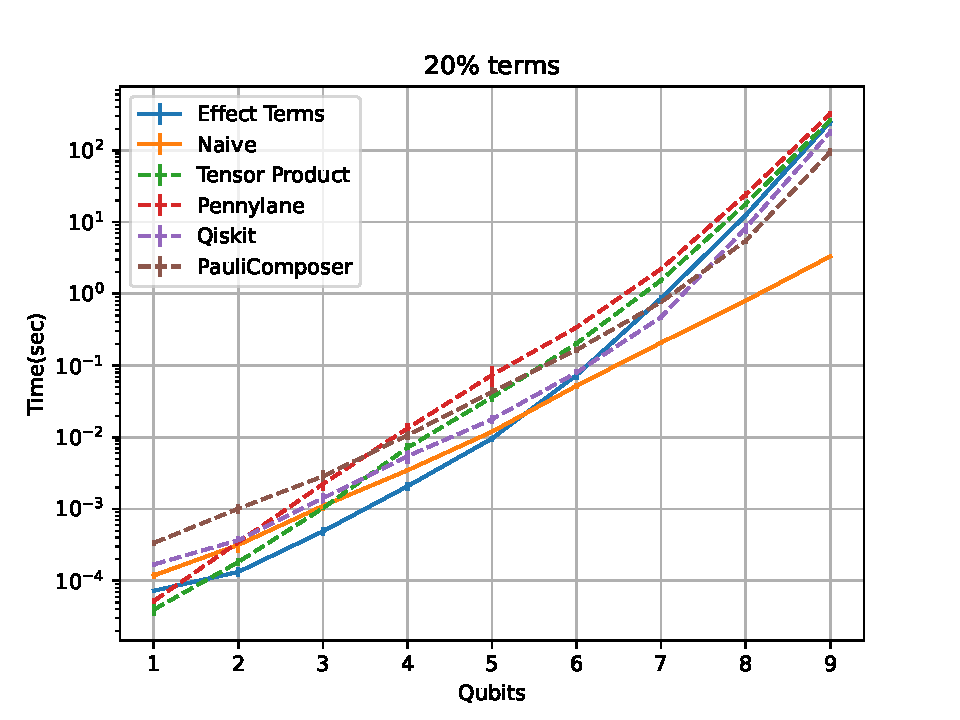
\includegraphics[width=0.5\linewidth]{0.2_terms.pdf}}
    \hfil
        \subfloat[]{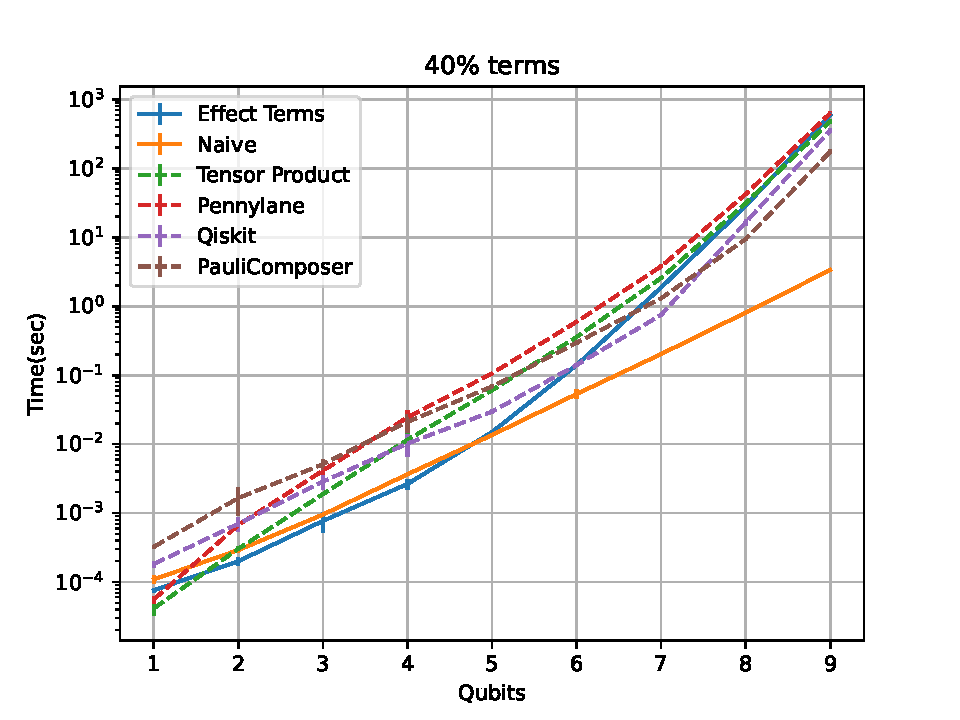
\includegraphics[width=0.5\linewidth]{0.4_terms.pdf}}
    
        \subfloat[]{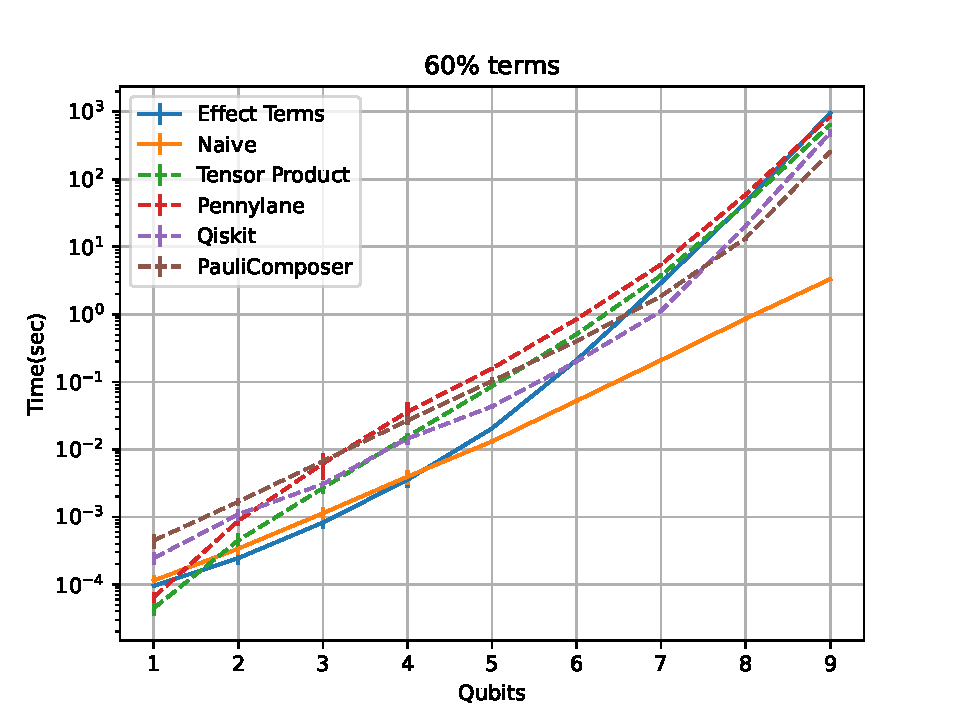
\includegraphics[width=0.5\linewidth]{0.6_terms.pdf}}
    \hfil
        \subfloat[]{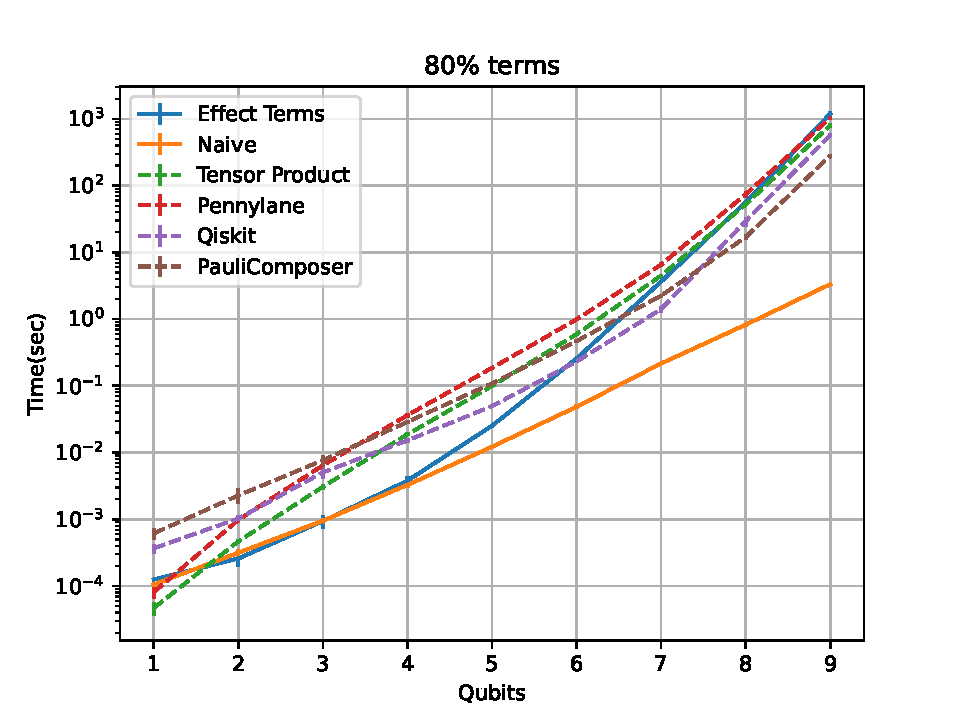
\includegraphics[width=0.5\linewidth]{0.8_terms.pdf}}
    
        \subfloat[]{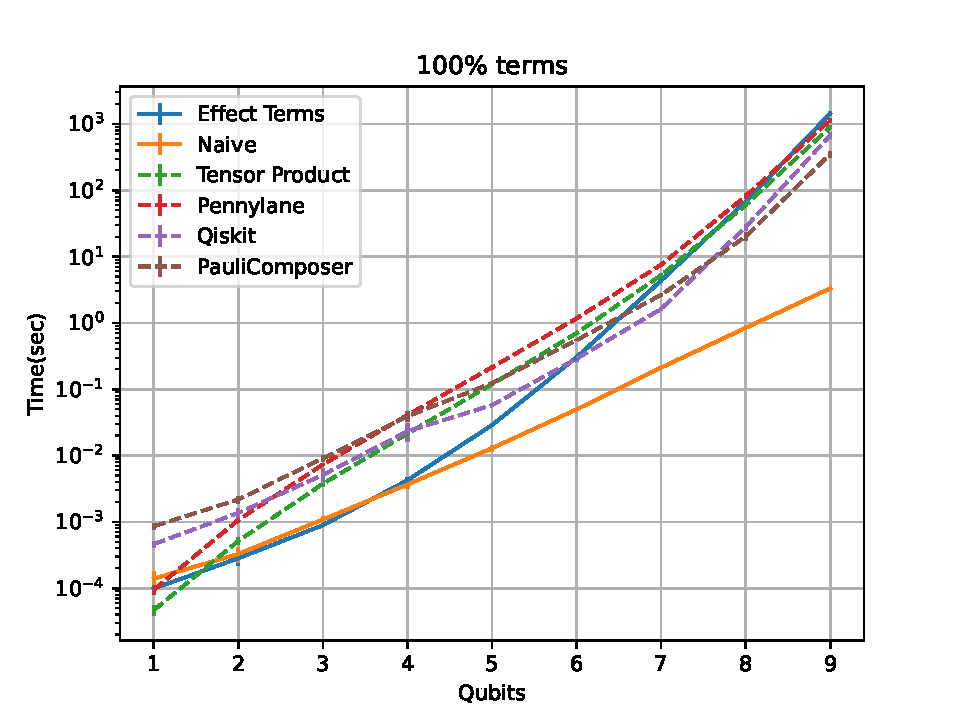
\includegraphics[width=0.5\linewidth]{1_terms.pdf}}
    \caption{Benchmarks for matrix composition of Puali polynomials with the algorithm \ref{alg:naive_inverse}, \ref{alg:effective_terms} with 
    Qiskit, Pennylane, PauliComposer, and standard tensor product methods, for $n=1$ to $n=9$. 
    The percentages of the each case represents how many coefficients are non-empty in $4^n$ number of spaces.}
        \label{fig:results}
\end{figure*}

\section{Conclusion}
We showed that the tensorized decomposition algorithm was a 
sequential basis transformation of the given matrix.
The common XZ simplex representation is one type of the transformation.
A simple conversion between the simplex representation and an index of the coefficient matrix 
where the output result the original decomposition, TPD algorithm\cite{hantzko_tensorized_2023}, 
was invetigated and the inverse composition algorithms were desgined. 
First algorithm is a naive tensor composition algorithm by inversing the TPD and using coefficient matrix.
The other is an effective term algorithm by calculate non-zero coefficients during the iterative 
steps of the naive version.
The algorithms are designed to compose the multiple terms at once, 
so that archieves better computational complexity in Pauli polynomial composition, in time and spatial both. 
The naive composition algorithm consists of basis transformation mapping between 
the coefficient matrix and the original matrix representation.

Comparing to the previous term-by-term methods which have $O(16^n + 4^n(f(n)-1))$ complexity in the worts case, 
the naive algorithm is at least, twice faster than the common term-by-term methods  with $O(8^n)$ complexity. 
It means that we can construct the matrix with computational basis corresponding to the given 
Pauli-polynomial at process of the algorithm. 
The inverse algorithm could chasing an effective terms during the composition process. 
However, chasing routine requires many computational costs it is not efficient as much as the naive version,
and even comparable with the term-by-term methods with $O(n16^n)$ complexity in the worst case.

In addition, the composition speed comparsion between the current quantum computing frameworks, Qiskit, Pennylane, and naive
tensor product routines. 
The inverse composition algorithm showed better speed for all cases, single, multi, worst terms 
for from $n=2$ to $n=9$ qubit cases. 
The naive algorithm was 10 or 1000 times faster than term-by-term methods.
Practically, even though the $k$ is small, the naive version is comparable 
with the term-by-term methods. 
We assume that it is caused from the spatial complexity effect.
The effective term algorithm could chase the effective terms, however in the current stage the time-cost benefit 
was not noticiable in the implementation.

\section*{Acknowledgments}
The research was funded by Quantum Sapiens Human resources center.

\section*{Data and code available}
The research was conducted for sub module of OptTrot python package for 
fast manipulation and optimization routine for Hamiltonian.
The tested code and the packages are available on OptTrot repository.
The same version of the code in the paper is on 
Zenodo repository\cite{kim_2024_11048922}.
%Bibliography
\bibliographystyle{unsrt}  
\bibliography{references}  

\appendix
%\section{Basis choice of TPD}
%
%\subsection{Pauli operations with ij index}
%
%\textbf{Group addition}
%
%\begin{equation}
%    P_1 \cdot P_2 = P_3
%\end{equation}
%
%\begin{itemize}
%    \item $n_i^3 = n_i^2 {}^\wedge n_i^1$
%    \item $n_j^3 = n_j^2 {}^\wedge n_j^1$
%\end{itemize}
%\textbf{Tensor Product}
%
%\begin{equation}
%    P_1 \otimes P_2 = P_3
%\end{equation}
%\begin{itemize}
%    \item $n_i^3 = (2^m n_i^2) \vee n_i^1$
%    \item $n_j^3 = (2^m n_j^2) \vee n_j^1$
%\end{itemize}

\section{Computational aspects}
In real implementation, the chasing the efficient calculation term during 
the algorithm requires huge time complexity.
The current implementation use bitwise operation, since, Python is not good for 
manipulate binary data, efficiently\footnote{Bitwise operators are even slower than string manipulation in Python.}. 
The above routines would be more appropriate for C/C++ or Rust like language implementation.
We could observe that the binary compiled routines did not show difference 
whether the algorithm has a effective term chasing routine or not.
Now, in python or the other interpreter language. It is wise to use the naive algorithm.
and if the language environment naturally manipulate the bits, the effective term chasing version
would be more appropriate.

%\end{multicols*}
\end{document}
